%=======================================================================
%  WEEKLY REPORT — LaTeX TEMPLATE
%  Cấu trúc: 1) Executive Summary  2) Completed Tasks  3) Results &
%            Visualization  4) Issues  5) Next Week Plan  6) References
%
%  Compile:  latexmk -pdf main.tex      (hoặc pdflatex 2 lần)
%  Tiếng Việt: file đã tự dò T5 encoding. Nếu vẫn lỗi dấu, dùng
%              xelatex/lualatex (nhánh fontspec bên dưới tự kích hoạt).
%
%  ---------------------- CHEAT SHEET NHANH -------------------------
%  \badge{ok}{Done}            → nhãn màu (ok / warn / bad / neutral)
%  \pbar{60}                   → thanh tiến độ 60%
%  \takeaway{...}              → 1–2 câu giải thích bắt buộc dưới hình/bảng
%  \evi{url}{label}            → link bằng chứng (commit/PR/notebook)
%  \ph[width]{text}            → ảnh placeholder, thay bằng \includegraphics
%  \begin{issuebox}{Title}     → khung mô tả một issue
%  Mọi mẫu định dạng (ảnh đôi, ảnh+bảng, text quấn ảnh, công thức,
%  biểu đồ, code, bullet lồng nhau) đều nằm ở Section 3.
%=======================================================================

\documentclass[11pt,a4paper]{article}

%------------------------ Encoding & font -----------------------------
\usepackage{iftex}
\ifPDFTeX
  \usepackage[utf8]{inputenc}
  % T5 = bảng mã tiếng Việt (gói vntex). Nếu máy không có, tự lùi về T1.
  \IfFileExists{t5enc.def}{\usepackage[T5]{fontenc}}{\usepackage[T1]{fontenc}}
  \IfFileExists{lmodern.sty}{\usepackage{lmodern}}{}
\else
  \usepackage{fontspec}
  \setmainfont{Latin Modern Roman}
  \setsansfont{Latin Modern Sans}
  \setmonofont{Latin Modern Mono}
\fi
\usepackage{microtype}

%------------------------ Layout --------------------------------------
\usepackage[a4paper,margin=2.3cm,top=2.6cm,bottom=2.4cm]{geometry}
\usepackage{fancyhdr}
\usepackage{lastpage}
\usepackage{titlesec}
\usepackage{setspace}
\setstretch{1.06}

%------------------------ Nội dung & hình ảnh -------------------------
\usepackage{graphicx}
\usepackage{float}          % [H] = ghim hình đúng vị trí
\usepackage{subcaption}     % 2 ảnh so sánh cạnh nhau
\usepackage{wrapfig}        % văn bản quấn quanh ảnh
\usepackage{caption}
\usepackage{booktabs}       % bảng 3 vạch chuẩn học thuật
\usepackage{tabularx}
\usepackage{longtable}
\usepackage{multirow}
\usepackage{array}
\usepackage{amsmath,amssymb}
\usepackage{enumitem}
\usepackage{xcolor}
\usepackage{listings}
\usepackage{tikz}
\usepackage{pgfplots}
\pgfplotsset{compat=1.18}
\usetikzlibrary{arrows.meta,positioning,shapes.geometric,calc}
\usepackage[most]{tcolorbox}
\tcbuselibrary{skins,breakable}

%------------------------ Bảng màu ------------------------------------
\definecolor{accent}{HTML}{2F6FBF}
\definecolor{accentdark}{HTML}{1B4A85}
\definecolor{ok}{HTML}{2E8B57}
\definecolor{warn}{HTML}{C98A00}
\definecolor{bad}{HTML}{C0392B}
\definecolor{neutral}{HTML}{6C757D}
\definecolor{rulegray}{HTML}{D5DAE0}

\usepackage[colorlinks=true,allcolors=accentdark,pdfusetitle]{hyperref}

%------------------------ METADATA (sửa ở đây) ------------------------
\newcommand{\ProjectName}{Benchmarking Stream Clustering Algorithms in River}
\newcommand{\WeekNo}{3}
\newcommand{\TotalWeeks}{18}
\newcommand{\WeekRange}{08 Jun 2026 \textendash{} 14 Jun 2026}
\newcommand{\AuthorName}{Nguyen Van A}
\newcommand{\MentorName}{Dr. B, Dr. C}
\newcommand{\PhaseName}{Phase 1 — Benchmark foundation}
\newcommand{\RepoURL}{https://github.com/user/repo}

%------------------------ Header / footer -----------------------------
\pagestyle{fancy}
\fancyhf{}
\renewcommand{\headrulewidth}{0.4pt}
\renewcommand{\footrulewidth}{0pt}
\fancyhead[L]{\small\color{neutral}\ProjectName}
\fancyhead[R]{\small\color{neutral}Week \WeekNo/\TotalWeeks}
\fancyfoot[C]{\small\color{neutral}\thepage\ / \pageref{LastPage}}

%------------------------ Style tiêu đề mục ---------------------------
\titleformat{\section}
  {\normalfont\large\bfseries\color{accentdark}}{\thesection.}{0.6em}{}
  [{\color{rulegray}\titlerule[0.8pt]}]
\titleformat{\subsection}
  {\normalfont\normalsize\bfseries\color{accentdark}}{\thesubsection}{0.6em}{}
\titlespacing*{\section}{0pt}{16pt}{7pt}
\titlespacing*{\subsection}{0pt}{10pt}{4pt}

\captionsetup{font=small,labelfont={bf,color=accentdark},skip=6pt}
\captionsetup[sub]{font=small}
\setlist[itemize]{itemsep=2pt,topsep=3pt,parsep=0pt,leftmargin=1.3em}
\setlist[enumerate]{itemsep=2pt,topsep=3pt,parsep=0pt,leftmargin=1.5em}

%------------------------ Macro tiện dụng -----------------------------
% Nhãn trạng thái: \badge{ok}{Done}, \badge{warn}{In progress}, ...
\newcommand{\badge}[2]{{\setlength{\fboxsep}{2.6pt}%
  \colorbox{#1!13}{\textcolor{#1!75!black}{\bfseries\footnotesize\MakeUppercase{#2}}}}}
\newcommand{\Done}{\badge{ok}{Done}}
\newcommand{\WIP}{\badge{warn}{In progress}}
\newcommand{\Blocked}{\badge{bad}{Blocked}}
\newcommand{\Planned}{\badge{neutral}{Planned}}

% Thanh tiến độ: \pbar{60}
\newcommand{\pbar}[1]{%
  \begin{tikzpicture}[baseline=-0.7ex]
    \fill[rulegray] (0,0) rectangle (1.7,0.2);
    \fill[accent]   (0,0) rectangle ({#1*0.017},0.2);
    \node[right,font=\scriptsize,text=black!70] at (1.78,0.1) {#1\%};
  \end{tikzpicture}\hspace*{1.6em}}

% Câu giải thích bắt buộc dưới mỗi hình/bảng
\newcommand{\takeaway}[1]{\par\vspace{-2pt}%
  \noindent{\small\itshape\color{black!72}\textbf{Takeaway.} #1}\par\vspace{6pt}}

% Link bằng chứng
\newcommand{\evi}[2]{\href{#1}{\texttt{\small #2}}}

% Ảnh placeholder — thay bằng \includegraphics khi có hình thật
\newcommand{\ph}[2][0.9\linewidth]{%
  \begin{tikzpicture}
    \node[draw=neutral!45,dashed,fill=neutral!7,rounded corners=2pt,
          minimum width=#1,minimum height={0.52*#1},align=center,
          inner sep=0pt,font=\ttfamily\small,text=neutral]{#2};
  \end{tikzpicture}}

% Khung mô tả issue
\newtcolorbox{issuebox}[1]{enhanced,breakable,
  colback=white,colframe=accent!40,boxrule=0.6pt,arc=2pt,
  left=7pt,right=7pt,top=5pt,bottom=5pt,
  fonttitle=\bfseries\small,coltitle=accentdark,colbacktitle=accent!8,
  title={#1}}

% Khung ghi chú / callout
\newtcolorbox{notebox}[1][Note]{enhanced,breakable,
  colback=ok!4,colframe=ok!45,boxrule=0.6pt,arc=2pt,
  fonttitle=\bfseries\small,coltitle=ok!70!black,colbacktitle=ok!10,title={#1}}

% Cột tabularx căn giữa / căn phải
\newcolumntype{C}[1]{>{\centering\arraybackslash}p{#1}}
\newcolumntype{R}{>{\raggedleft\arraybackslash}X}
\newcolumntype{L}{>{\raggedright\arraybackslash}X}

% Style cho code
\lstdefinestyle{py}{
  basicstyle=\ttfamily\footnotesize,
  keywordstyle=\color{accentdark}\bfseries,
  commentstyle=\color{ok!70!black}\itshape,
  stringstyle=\color{bad!80!black},
  numbers=left,numberstyle=\tiny\color{neutral},numbersep=7pt,
  backgroundcolor=\color{neutral!5},
  frame=single,rulecolor=\color{rulegray},
  breaklines=true,showstringspaces=false,
  xleftmargin=16pt,framexleftmargin=16pt,language=Python}

%=======================================================================
\begin{document}

%------------------------ TITLE BLOCK ---------------------------------
\begin{center}
  {\LARGE\bfseries\color{accentdark} Weekly Report \#\WeekNo\par}
  \vspace{3pt}
  {\large \ProjectName\par}
\end{center}
\vspace{4pt}

\noindent
\begin{tabularx}{\textwidth}{@{}>{\bfseries\small}l >{\small}X >{\bfseries\small}l >{\small}X@{}}
\toprule
Contributor & \AuthorName            & Reporting period & \WeekRange \\
Mentors     & \MentorName            & Phase            & \PhaseName \\
Repository  & \evi{\RepoURL}{github.com/user/repo} & Report date & \today \\
\bottomrule
\end{tabularx}
\vspace{6pt}

%=======================================================================
\section{Executive Summary}
%=======================================================================
\begin{description}[font=\bfseries\color{accentdark},style=sameline,leftmargin=0pt,labelindent=0pt,itemindent=0pt,labelwidth=0pt,labelsep=0.4em,
                    itemsep=4pt,topsep=2pt]
  \item[Objective —] Establish the core benchmark metrics suite for stream
        clustering, so that every algorithm added later can be scored with
        one unified, reproducible interface (maps to \PhaseName, milestone~P1.2).

  \item[Status —] \Done\ \textbf{On Track} — the metric selection and the
        evaluation protocol were finalised on schedule; the calculation
        script is 60\% implemented and no blocker has appeared.

  \item[Self-assessment —] $\approx$\,85\% of the weekly plan completed.
        Quality is good on the design side (metrics are justified against
        literature), weaker on the engineering side: the incremental
        silhouette implementation still lacks unit tests.
\end{description}

\subsection*{Progress tracker}

\begin{table}[H]
\centering
\caption{Weekly plan versus reality, week \WeekNo.}
\label{tab:tracker}
\small
\begin{tabularx}{\textwidth}{@{}L c l l@{}}
\toprule
\textbf{Weekly plan item} & \textbf{Phase ref.} & \textbf{Status} & \textbf{Completion} \\
\midrule
Select metrics suite (ARI, purity, silhouette, throughput) & P1.2 & \Done    & \pbar{100} \\
Write metric calculation script                            & P1.2 & \WIP     & \pbar{60}  \\
Draft benchmark pipeline architecture                      & P1.3 & \Done    & \pbar{100} \\
Unit tests for incremental silhouette                      & P1.2 & \Planned & \pbar{0}   \\
\bottomrule
\end{tabularx}
\end{table}
\takeaway{Only the testing task slipped to next week; it is not on the critical
path because the pipeline skeleton (P1.3) does not depend on it.}

\noindent\textbf{Overall:} Week \WeekNo/\TotalWeeks{} — on schedule.

%=======================================================================
\section{Completed Tasks}
%=======================================================================
\begin{enumerate}[label=\textbf{C\arabic*.},leftmargin=2.2em]
  \item \textbf{Surveyed the internal design of River's clustering module}
        \hfill{\small(P1.1)}\\
        Summarised how \texttt{CluStream} and \texttt{DenStream} are
        implemented in River and identified \textbf{3 structural differences}:
        (i) micro-cluster storage (fixed array vs.\ dynamic dict),
        (ii) decay handling (time-window vs.\ exponential fading), and
        (iii) the absence of a common \texttt{predict\_one} contract for
        outlier points.
        \emph{Evidence:} \evi{\RepoURL/blob/main/notes/river-internals.md}{notes/river-internals.md},
        \evi{\RepoURL/commit/a1b2c3d}{commit a1b2c3d}.

  \item \textbf{Finalised the metric suite and its justification}
        \hfill{\small(P1.2)}\\
        4 metrics selected out of 11 candidates; each one mapped to a
        concrete failure mode it detects (see Table~\ref{tab:metrics}).
        \emph{Evidence:} \evi{\RepoURL/pull/12}{PR \#12}.

  \item \textbf{Implemented \texttt{MetricRegistry} and 2 of 4 metrics}
        \hfill{\small(P1.2)}\\
        ARI and purity run incrementally over a stream of 100k points in
        \textbf{1.9\,s} with a constant memory footprint of $\approx$\,12\,MB.
        \emph{Evidence:} \evi{\RepoURL/blob/main/bench/metrics.py}{bench/metrics.py}.
\end{enumerate}

\subsection*{In progress}
\begin{itemize}
  \item \WIP\ \textbf{Incremental silhouette} (60\%) — the sampling-based
        approximation works, but the error bound versus the exact score is
        still unmeasured. Expected completion: Mon of week \number\numexpr\WeekNo+1\relax.
  \item \Planned\ \textbf{Unit tests + CI hook} (0\%) — moved to next week,
        deliberately, to keep the metric API stable first.
\end{itemize}

\subsection*{Time log}
\noindent\small
Research River internals: \textbf{6h} $\cdot$ Metric selection \& write-up:
\textbf{3h} $\cdot$ Implement metric script: \textbf{4h} $\cdot$ Concept-drift
reading: \textbf{2h} $\cdot$ Mentor sync \& report: \textbf{1.5h}
\quad$\Rightarrow$\quad\textbf{Total: 16.5h}.
\normalsize\par
% Bản chi tiết theo ngày nằm ở Appendix A.

%=======================================================================
\section{Results \& Visualization}
%=======================================================================
% GHI CHÚ: mọi hình/bảng đều phải có caption + \takeaway{...}.
% Section này chứa TẤT CẢ các mẫu định dạng — xoá mẫu nào không dùng.

%-------------------------------------------------- 3.1 sơ đồ TikZ ----
\subsection{Benchmark pipeline architecture}

\begin{figure}[H]
\centering
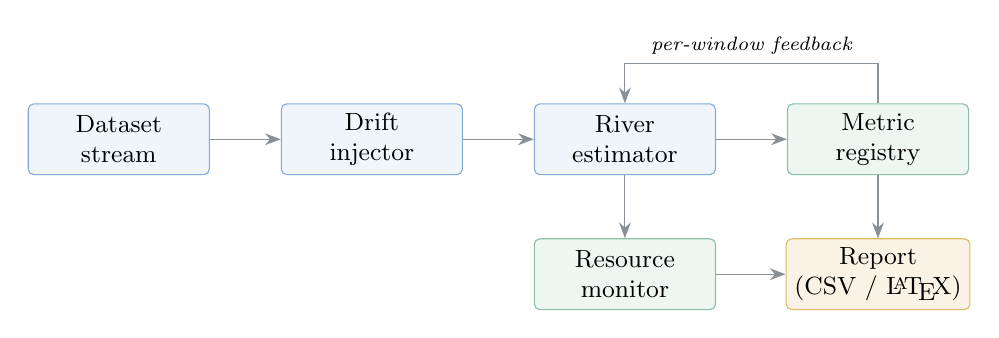
\begin{tikzpicture}[
  node distance=8mm and 9mm,
  box/.style={draw=accent!60,fill=accent!7,rounded corners=2pt,
              minimum height=9mm,minimum width=23mm,align=center,
              font=\small,inner sep=3pt},
  store/.style={box,fill=ok!8,draw=ok!55},
  outbox/.style={box,fill=warn!10,draw=warn!60},
  arr/.style={-{Stealth[length=2mm]},draw=neutral!80}]

  \node[box] (src)   {Dataset\\stream};
  \node[box,right=of src] (drift) {Drift\\injector};
  \node[box,right=of drift] (algo) {River\\estimator};
  \node[store,right=of algo] (met) {Metric\\registry};
  \node[outbox,below=of met] (rep) {Report\\(CSV / \LaTeX)};
  \node[store,below=of algo] (res) {Resource\\monitor};

  \draw[arr] (src) -- (drift);
  \draw[arr] (drift) -- (algo);
  \draw[arr] (algo) -- (met);
  \draw[arr] (met) -- (rep);
  \draw[arr] (algo) -- (res);
  \draw[arr] (res) -- (rep);
  \draw[arr] (met.north) -- ++(0,5mm) -| node[pos=0.25,above,font=\scriptsize\itshape]
       {per-window feedback} (algo.north);
\end{tikzpicture}
\caption{Proposed benchmark pipeline. Each block is a swappable component
         behind a single interface.}
\label{fig:pipeline}
\end{figure}
\takeaway{Decoupling the drift injector from the estimator means the same
algorithm can be re-run under different drift regimes without touching the
scoring code, which is what makes the benchmark reproducible.}

%-------------------------------------------- 3.2 công thức + bảng ----
\subsection{Metric definitions}

The internal quality of a partition is measured with the silhouette score.
For a point $i$ with mean intra-cluster distance $a(i)$ and mean nearest-cluster
distance $b(i)$:
\begin{equation}
  s(i) \;=\; \frac{b(i) - a(i)}{\max\{a(i),\,b(i)\}},
  \qquad s(i) \in [-1, 1],
  \label{eq:silhouette}
\end{equation}
and the score of the stream window $W$ is the running mean
$\bar{s}_W = \frac{1}{|W|}\sum_{i \in W} s(i)$.

External agreement uses the adjusted Rand index, which corrects the raw Rand
index for chance:
\begin{align}
  \mathrm{ARI}
  &= \frac{\displaystyle\sum_{ij}\binom{n_{ij}}{2}
           - \Big[\sum_i\binom{a_i}{2}\sum_j\binom{b_j}{2}\Big] \big/ \binom{n}{2}}
          {\displaystyle\frac{1}{2}\Big[\sum_i\binom{a_i}{2}+\sum_j\binom{b_j}{2}\Big]
           - \Big[\sum_i\binom{a_i}{2}\sum_j\binom{b_j}{2}\Big] \big/ \binom{n}{2}}
  \label{eq:ari}
\end{align}
where $n_{ij}$ is the contingency count, $a_i$ and $b_j$ the row/column sums.

\begin{table}[H]
\centering
\caption{Selected metrics and the reason each one is included.}
\label{tab:metrics}
\small
\begin{tabularx}{\textwidth}{@{}l c c L@{}}
\toprule
\textbf{Metric} & \textbf{Type} & \textbf{Range} & \textbf{Why it is in the suite} \\
\midrule
ARI (Eq.~\ref{eq:ari})        & External & $[-1,1]$ & Chance-corrected; comparable across datasets with different cluster counts. \\
Purity                        & External & $[0,1]$  & Cheap to compute online; exposes majority-class collapse that ARI can hide. \\
Silhouette (Eq.~\ref{eq:silhouette}) & Internal & $[-1,1]$ & The only metric usable when ground-truth labels are unavailable. \\
Throughput                    & System   & pts/s    & Stream algorithms are useless if they cannot keep up with the arrival rate. \\
\bottomrule
\end{tabularx}
\end{table}
\takeaway{The suite deliberately mixes external, internal and system metrics:
an algorithm that wins on ARI but processes 200 points/s would fail the real
use case, and the table makes that trade-off visible in one place.}

%--------------------------------------------------- 3.3 một ảnh ------
\subsection{Single figure}

\begin{figure}[H]
\centering
% THAY BẰNG: \includegraphics[width=0.72\linewidth]{figures/clusters.png}
\ph[0.72\linewidth]{figures/clusters.png}
\caption{Clustering result of CluStream on the \texttt{sea} dataset after
         50k points.}
\label{fig:single}
\end{figure}
\takeaway{Micro-clusters stay well separated in the first two dimensions, which
confirms the radius parameter chosen in week 2 is still appropriate at this
stream length.}

%------------------------------------------ 3.4 hai ảnh so sánh -------
\subsection{Side-by-side comparison}

\begin{figure}[H]
\centering
\begin{subfigure}[b]{0.48\linewidth}
  \centering
  % \includegraphics[width=\linewidth]{figures/before_drift.png}
  \ph[\linewidth]{before\_drift.png}
  \caption{Before drift ($t < 25$k)}
  \label{fig:before}
\end{subfigure}\hfill
\begin{subfigure}[b]{0.48\linewidth}
  \centering
  % \includegraphics[width=\linewidth]{figures/after_drift.png}
  \ph[\linewidth]{after\_drift.png}
  \caption{After drift ($t > 25$k)}
  \label{fig:after}
\end{subfigure}
\caption{Cluster layout before and after an abrupt concept drift, same
         algorithm and same parameters.}
\label{fig:compare}
\end{figure}
\takeaway{The right-hand panel shows two micro-clusters that were never merged
after the drift, i.e.\ the fading factor reacts too slowly — this is the
motivation for issue~I1 below.}

%---------------------------------------- 3.5 ảnh + bảng cạnh nhau ----
\subsection{Figure next to a table}

\begin{figure}[H]
\centering
\begin{minipage}[t]{0.46\linewidth}
  \centering
  \vspace{0pt}
  % \includegraphics[width=\linewidth]{figures/memory.png}
  \ph[\linewidth]{memory\_profile.png}
  \captionof{figure}{Memory profile over the stream.}
  \label{fig:mem}
\end{minipage}\hfill
\begin{minipage}[t]{0.5\linewidth}
  \vspace{0pt}
  \centering
  \captionof{table}{Peak resource usage.}
  \label{tab:mem}
  \small
  \begin{tabular}{@{}lrr@{}}
  \toprule
  \textbf{Algorithm} & \textbf{Peak RAM} & \textbf{pts/s} \\
  \midrule
  CluStream     & 41\,MB & 12\,400 \\
  DenStream     & 78\,MB &  6\,900 \\
  STREAMKMeans  & 19\,MB & 21\,800 \\
  \bottomrule
  \end{tabular}
\end{minipage}
\end{figure}
\takeaway{DenStream costs roughly twice the memory of CluStream for a lower
throughput; unless its quality advantage is large, it is the weakest candidate
for the memory-constrained scenario in the proposal.}

%----------------------------------- 3.6 văn bản quấn quanh ảnh -------
\subsection{Text wrapped around a figure}

\begin{wrapfigure}{r}{0.35\linewidth}
  \vspace{-8pt}
  \centering
  % \includegraphics[width=\linewidth]{figures/microcluster.png}
  \ph[\linewidth]{microcluster.png}
  \caption{Micro-cluster radius growth.}
  \label{fig:wrap}
  \vspace{-6pt}
\end{wrapfigure}

Use this layout when the figure is small and the surrounding explanation is
what actually matters. Figure~\ref{fig:wrap} tracks the mean micro-cluster
radius across the stream; the radius grows monotonically until the first
merge event, then stabilises. The important detail is the plateau after
$t = 30$k: it means the structure has converged and any later change is
caused by drift rather than by initialisation noise. Keep at least four or
five lines of text next to a wrapped figure, otherwise the layout looks
broken and it is better to fall back to a normal centred figure.

%--------------------------------------------- 3.7 bảng kết quả -------
\subsection{Full result table}

\begin{table}[H]
\centering
\caption{Benchmark results on 3 datasets. Best value per column in \textbf{bold}.}
\label{tab:results}
\small
\begin{tabular}{@{}l cc cc cc@{}}
\toprule
& \multicolumn{2}{c}{\textbf{sea}} & \multicolumn{2}{c}{\textbf{covtype}}
& \multicolumn{2}{c}{\textbf{insects}} \\
\cmidrule(lr){2-3}\cmidrule(lr){4-5}\cmidrule(lr){6-7}
\textbf{Algorithm} & ARI & Sil. & ARI & Sil. & ARI & Sil. \\
\midrule
CluStream    & \textbf{0.71} & 0.55 & \textbf{0.63} & \textbf{0.48} & 0.52 & 0.41 \\
DenStream    & 0.64 & 0.49 & 0.58 & 0.44 & \textbf{0.61} & \textbf{0.47} \\
STREAMKMeans & 0.58 & \textbf{0.61} & 0.55 & 0.46 & 0.44 & 0.38 \\
\midrule
\multicolumn{7}{@{}l@{}}{\footnotesize Mean of 5 runs, window $=1000$, seed
$\in\{1..5\}$. Std.\ dev.\ $< 0.03$ everywhere.} \\
\bottomrule
\end{tabular}
\end{table}
\takeaway{No algorithm dominates on all datasets: CluStream leads on the two
synthetic streams while DenStream wins on the real, noisier \texttt{insects}
data, which suggests noise robustness — not raw accuracy — is the property
worth isolating in week 4.}

%---------------------------------------------- 3.8 biểu đồ ----------
\subsection{Performance chart}

\begin{figure}[H]
\centering
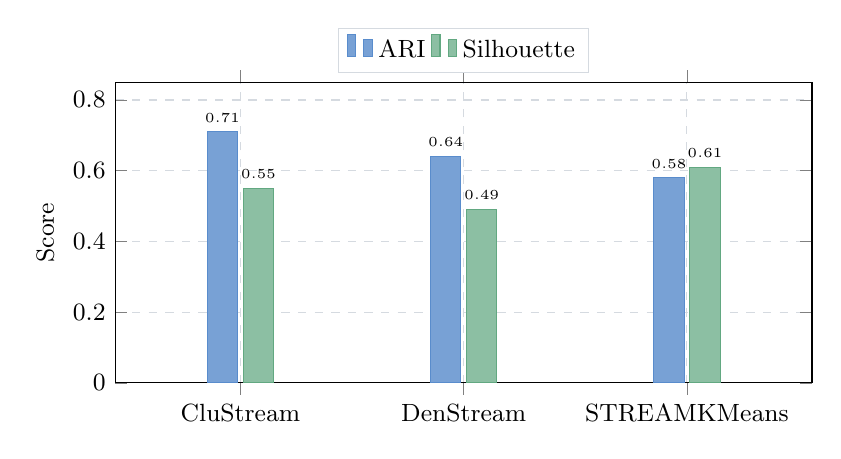
\begin{tikzpicture}
\begin{axis}[
  ybar, width=0.86\linewidth, height=5.4cm,
  bar width=11pt, enlarge x limits=0.28,
  symbolic x coords={CluStream,DenStream,STREAMKMeans},
  xtick=data, ymin=0, ymax=0.85,
  ylabel={Score}, ylabel style={font=\small},
  tick label style={font=\small},
  legend style={at={(0.5,1.03)},anchor=south,legend columns=-1,
                font=\small,draw=rulegray},
  nodes near coords, every node near coord/.append style={font=\tiny},
  grid=major, grid style={rulegray,dashed}]
  \addplot[fill=accent!65,draw=accent!80] coordinates
    {(CluStream,0.71) (DenStream,0.64) (STREAMKMeans,0.58)};
  \addplot[fill=ok!55,draw=ok!75] coordinates
    {(CluStream,0.55) (DenStream,0.49) (STREAMKMeans,0.61)};
  \legend{ARI, Silhouette}
\end{axis}
\end{tikzpicture}
\caption{External (ARI) versus internal (silhouette) agreement on the
         \texttt{sea} dataset.}
\label{fig:chart}
\end{figure}
\takeaway{STREAMKMeans has the best silhouette but the worst ARI — a textbook
sign that it produces geometrically tidy clusters that do not match the true
labels, so silhouette alone must never be used as the selection criterion.}

%---------------------------------------------- 3.9 code snippet ------
\subsection{Reference implementation snippet}

\begin{lstlisting}[style=py,caption={Incremental metric update loop.},
                   label={lst:loop}]
for x, y_true in stream:
    y_pred = model.predict_one(x)      # score before learning
    for metric in registry:            # ARI, purity, silhouette, ...
        metric.update(y_true, y_pred)
    model.learn_one(x)
    if i % WINDOW == 0:
        snapshot(registry, step=i)     # one row per window
\end{lstlisting}
\takeaway{Scoring strictly before \texttt{learn\_one} is what makes the
protocol prequential; reversing the two lines would leak the current point
into the model and inflate every metric.}

%---------------------------------------------- 3.10 bullet mẫu -------
\subsection{Observations}

\begin{itemize}
  \item \textbf{Parameter sensitivity.} CluStream reacts strongly to the
        micro-cluster count $q$:
        \begin{itemize}
          \item $q = 50$ — clusters merge too early, ARI drops by $0.09$;
          \item $q = 200$ — quality plateaus, memory grows linearly;
          \item $q = 100$ — chosen default, best quality/memory ratio.
        \end{itemize}
  \item \textbf{Drift response.} Recovery after an abrupt drift takes
        $\approx 3$ windows for CluStream and $\approx 7$ for DenStream.
  \item \textbf{Reproducibility.} All runs are seeded; re-running
        \texttt{make bench} reproduces Table~\ref{tab:results} bit-for-bit.
\end{itemize}

\begin{notebox}[Design decision]
Silhouette is computed on a reservoir sample of 2\,000 points per window
instead of the full window. Exact computation is $O(n^2)$ and would dominate
the runtime of the benchmark itself, defeating the purpose of the throughput
metric.
\end{notebox}

%=======================================================================
\section{Issues}
%=======================================================================
% Nếu tuần trơn tru: xoá các issuebox và ghi rõ dòng dưới đây.
% \noindent\textbf{No major blockers this week.}

\begin{issuebox}{I1 — Fading factor reacts too slowly after abrupt drift}
\begin{description}[font=\bfseries,style=sameline,leftmargin=0pt,labelindent=0pt,itemindent=0pt,labelwidth=0pt,labelsep=0.4em,itemsep=2pt,topsep=2pt]
  \item[Type:] Technical / algorithmic.
  \item[Impact:] \badge{warn}{Medium} — biases the drift-recovery numbers
        planned for week 5, but does not block the current phase.
  \item[Handling:] Reproduced with a minimal script
        (\evi{\RepoURL/issues/7}{issue \#7}); tested $\lambda \in \{0.25, 0.5, 1.0\}$
        and confirmed the effect is parameter-driven, not a bug in River.
  \item[Mentor support:] Not needed yet. I will propose a fixed $\lambda$
        grid in the week-4 report and only escalate if the grid cannot
        separate algorithm behaviour from parameter behaviour.
\end{description}
\end{issuebox}

\begin{issuebox}{I2 — Ambiguity about which drift definition the proposal targets}
\begin{description}[font=\bfseries,style=sameline,leftmargin=0pt,labelindent=0pt,itemindent=0pt,labelwidth=0pt,labelsep=0.4em,itemsep=2pt,topsep=2pt]
  \item[Type:] Conceptual.
  \item[Impact:] \badge{bad}{High} — the choice between real and virtual
        drift changes which datasets belong in the benchmark suite.
  \item[Handling:] Read Gama et al.\ (2014) and drafted two candidate scopes
        with the datasets each one implies (\evi{\RepoURL/blob/main/notes/drift-scope.md}{notes/drift-scope.md}).
  \item[Mentor support:] \textbf{Yes} — a 10-minute decision at the next sync
        would unblock the dataset list for Phase~2. My recommendation:
        cover real drift only, and treat virtual drift as a stretch goal.
\end{description}
\end{issuebox}

\begin{table}[H]
\centering
\caption{Issue summary.}
\label{tab:issues}
\small
\begin{tabularx}{\textwidth}{@{}l L c c l@{}}
\toprule
\textbf{ID} & \textbf{Short description} & \textbf{Type} & \textbf{Impact} & \textbf{Mentor input?} \\
\midrule
I1 & Slow fading response after drift & Technical  & \badge{warn}{Medium} & No \\
I2 & Drift definition scope unclear   & Conceptual & \badge{bad}{High}    & \textbf{Yes} \\
\bottomrule
\end{tabularx}
\end{table}
\takeaway{Only I2 needs a decision from the mentors; everything else has an
owner and a plan, so the sync can stay short.}

%=======================================================================
\section{Next Week's Plan}
%=======================================================================

\begin{table}[H]
\centering
\caption{Plan for week \number\numexpr\WeekNo+1\relax{} (\PhaseName{} → Phase 2 hand-off).}
\label{tab:next}
\small
\begin{tabularx}{\textwidth}{@{}c L L c@{}}
\toprule
\textbf{\#} & \textbf{Task} & \textbf{Definition of done (verifiable)} & \textbf{Phase} \\
\midrule
N1 & Finish incremental silhouette & Approximation error $< 0.02$ vs.\ exact score on 3 datasets, documented in the notebook & P1.2 \\
N2 & Unit tests + CI              & $\geq 90\%$ line coverage on \texttt{bench/metrics.py}, GitHub Actions green & P1.2 \\
N3 & Wire the full pipeline       & \texttt{make bench} runs end-to-end on 1 dataset and emits a CSV & P1.3 \\
N4 & Noise-robustness experiment  & Table of ARI at 0/5/10\% label noise for 3 algorithms & P2.1 \\
\bottomrule
\end{tabularx}
\end{table}
\takeaway{N3 is the milestone that closes Phase 1; N1 and N2 are the carry-over
items from this week and are scheduled first so the slip does not compound.}

\subsection*{Catch-up plan}
\begin{itemize}
  \item The two unfinished items (N1, N2) are front-loaded to Mon–Tue,
        before any new Phase-2 work starts.
  \item Estimated catch-up cost: 5h, absorbed inside the normal weekly budget
        — no schedule extension required.
\end{itemize}

\subsection*{Risks for next week}
\begin{itemize}
  \item If I2 is not resolved at the sync, N4 will be run on synthetic data
        only and re-run later once the scope is fixed.
\end{itemize}

%=======================================================================
\section{References / Links}
%=======================================================================

\subsection*{Code produced this week}
\begin{table}[H]
\centering
\small
\begin{tabularx}{\textwidth}{@{}l L l@{}}
\toprule
\textbf{Ref} & \textbf{Description} & \textbf{Link} \\
\midrule
PR \#12      & Metric suite + registry            & \evi{\RepoURL/pull/12}{pull/12} \\
\texttt{a1b2c3d} & River internals write-up       & \evi{\RepoURL/commit/a1b2c3d}{commit} \\
\texttt{feat/metrics} & Working branch            & \evi{\RepoURL/tree/feat/metrics}{branch} \\
Notebook     & Metric sanity checks               & \evi{\RepoURL/blob/main/nb/01-metrics.ipynb}{nb/01-metrics.ipynb} \\
\bottomrule
\end{tabularx}
\end{table}

\subsection*{Datasets}
\begin{itemize}
  \item \textbf{SEA} (synthetic, 100k pts) — generated with
        \texttt{river.datasets.synth.SEA}, seed 42.
  \item \textbf{Covertype} (581k pts) — UCI Machine Learning Repository,
        \evi{https://archive.ics.uci.edu/dataset/31/covertype}{archive.ics.uci.edu/dataset/31}.
  \item \textbf{INSECTS} (abrupt variant) — USP data stream repository.
\end{itemize}

\subsection*{Literature and documentation}
\begin{thebibliography}{9}
\small
\bibitem{gama2014} J.~Gama et al., ``A survey on concept drift adaptation,''
  \emph{ACM Computing Surveys}, 46(4), 2014.
\bibitem{aggarwal2003} C.~C. Aggarwal et al., ``A framework for clustering
  evolving data streams,'' \emph{VLDB}, 2003.
\bibitem{cao2006} F.~Cao et al., ``Density-based clustering over an evolving
  data stream with noise,'' \emph{SDM}, 2006.
\bibitem{riverdocs} River documentation, \emph{Clustering module},
  \url{https://riverml.xyz}.
\end{thebibliography}
% Nếu muốn dùng BibTeX: thay khối trên bằng
% \bibliographystyle{plain}\bibliography{refs}

%=======================================================================
\appendix
\section{Detailed time log}
%=======================================================================

\begin{longtable}{@{}l p{8.1cm} l r@{}}
\caption{Hours logged per day, week \WeekNo.}\label{tab:timelog}\\
\toprule
\textbf{Date} & \textbf{Activity} & \textbf{Category} & \textbf{Hours} \\
\midrule
\endfirsthead
\multicolumn{4}{@{}l}{\small\itshape Table~\ref{tab:timelog} (continued)}\\
\toprule
\textbf{Date} & \textbf{Activity} & \textbf{Category} & \textbf{Hours} \\
\midrule
\endhead
\midrule
\multicolumn{4}{r@{}}{\small\itshape continued on next page}\\
\endfoot
\midrule
\textbf{Total} & & & \textbf{16.5} \\
\bottomrule
\endlastfoot
Mon 08 & Read River clustering source, take notes      & Research    & 4.0 \\
Tue 09 & Compare CluStream vs.\ DenStream internals    & Research    & 2.0 \\
Tue 09 & Shortlist candidate metrics                   & Design      & 3.0 \\
Wed 10 & Implement \texttt{MetricRegistry}, ARI, purity& Engineering & 2.5 \\
Thu 11 & Incremental silhouette (partial)              & Engineering & 1.5 \\
Thu 11 & Concept-drift literature                      & Research    & 2.0 \\
Fri 12 & Mentor sync + write this report               & Admin       & 1.5 \\
\end{longtable}

\end{document}
